\chapter{Graphs and Algorithms} \label{algorithms}

With the problem statement formalised in the previous section \ref{problem_statement}, we will now discuss the graph data structure and the algorithms which could potentially assist in solving the 15-Minute City problem.

\section{Graphs}

Graph is a mathematical data structure in Graph Theory representing pairwise relationships between objects. The earliest scientiifc paper was the ``Seven Bridges of Königsberg'' by Leonhard Euler published in the $18^{th}$ centry. The ``Seven Bridges of Königsberg'' was proven to have no solution to the problem of crossing each of the seven bridges exactly once and returning to the starting point. Euler represented the problem by a graph, where the land masses were represented by vertices and the bridges were represented by edges.

% \begin{figure}[H]
%     \centering
%     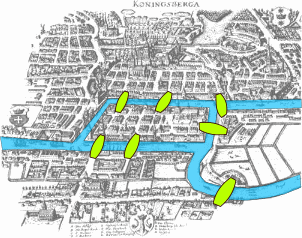
\includegraphics[width=0.6\textwidth]{Konigsberg_bridges.png}
%     \caption{Konigsberg Bridges}
%     \label{fig:konigsberg_bridges}
% \end{figure}\hfill

\begin{figure}[htbp]
    \centering
    \begin{subfigure}[c]{0.6\textwidth}
        % \centering
        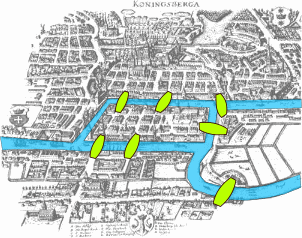
\includegraphics[width=\textwidth]{Konigsberg_bridges.png}
    \end{subfigure}\hfill
    \begin{subfigure}[c]{0.4\textwidth}
        % \centering
        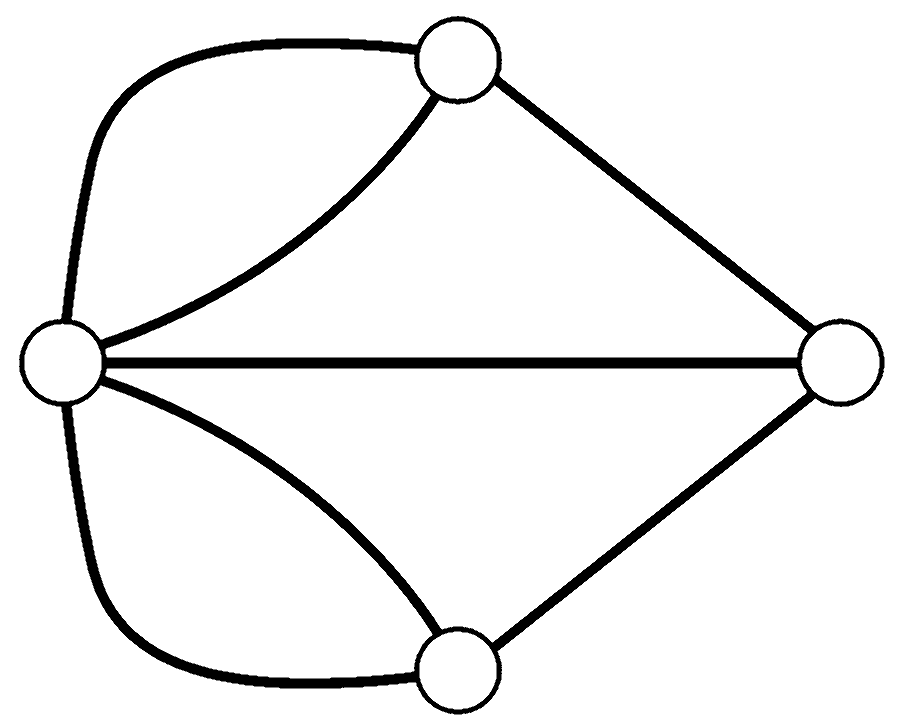
\includegraphics[width=\textwidth]{Konigsberg_bridges_graph.png}
    \end{subfigure} \hfill
    \caption{Konigsberg Bridges and its graph representation}
    \label{fig:konigsberg_bridges}
\end{figure}

In general, a graph can be defined as $G(V,E)$, where $V$ is the set of vertices and $E\subseteq V\times V$ is the set of edges. The edges can be directed or undirected, and weighted or unweighted. Labels can also be assigned to the vertices and edges, which can be used to represent additional information about the graph. For example, in ``Seven Bridges of Königsberg'', the vertices could be labelled with the names of the islands/areas and the edges could be labelled with the names of bridges. Furthermore, the edges could be weighted with the length of the bridges.

\section{Graph Search Algorithms}

In this section, we will discuss 3 types of graph search algorithms, the graph traversal problem, minimum spanning tree and the shortest path problem. The graph traversal problem is a problem of visiting all the nodes in a graph, while the shortest path problem is a problem of finding the shortest path between two nodes in a graph. The algorithms discussed in this section are fundamental graph algorithms and we will discuss their characteristics, properties, and whether they are suitable for solving the 15-Minute City problem.

\subsection{Graph Traversal Problem}

The Graph Traversal Problem is a problem of visiting all the nodes in a graph. There are two types of graph traversal algorithms, Breadth-First Search (BFS) and Depth-First Search (DFS). Both algorithms can be used to search for connected components of a graph and search for cycles, and have complexity $\mathcal{O}(V+E)$.

\subsubsection{Breadth-first Search (BFS)}

Breadth-first Search algorithm is a single-source graph search algorithm where the graph contains unweighted, undirected edges. The algorithm searches the graph from the source node level by level, that means the algorithm will search all nodes adjacent to the source node, before moving on to searching all nodes adjacent to these nodes. The visited nodes will be marked so that the algorithm will not be stuck in a cycle. An example of an application of this algorithm is maze solving, where it can be used to find the shortest path through a maze from the source node (i.e. entrance/exit).

\subsubsection{Depth-First Search (DFS)}

Depth-First Search algorithm is another popular single-source graph search algorithm for graphs with unweighted, undirected edges. Depth-First Search starts from the source node, travels along one of its edges and visits the adjacent node, the algorithm then repeats the process to this adjacent node and so on. Once the algorithm gets to the final node (i.e. there are no edges connected to this node where the adjacent node has not been visited), the algorithm travels to the previous level and checks if that node has an alternate adjacent node through a different edge. This process is then repeated until all nodes have been visited which can be reached to from our source node. Similar to Breadth-first Search algorithm, this algorithm can be used to detect connected components of a graph and search for cycles.

\subsection{Minimum Spanning Tree}

Minimum Spanning Tree (MST) is a Graph Theory problem of finding a tree that connects all the nodes in a graph with the least possible total edge weight and without any cycles. There are several algorithms that can be used to solve the minimum spanning tree problem, such as Prim's algorithm and Kruskal's algorithm. These algorithms can be used to find the minimum spanning tree in a weighted, undirected graph.

\subsubsection{Prim's Algorithm}

Prim's algorithm is used for finding the MST within a weighted, undirected graph. Prim's algorithm starts from the source node, it keeps a record of the nodes it has selected. It repeatedly searches for the edge with the smallest weight that connects a node from the selected set of node and another node outside of this set. Prim's algorithm is a greedy algorithm and an example of an application is used in network design problems to find the minimum cost to connect all nodes in a network. The complexity of Prim's algorithm is $\mathcal{O}(|E|+|V|\log |V|)$.

\subsubsection{Kruskal's Algorithm}

Kruskal's algorithm is similar to Prim algorithm that it is a greedy algorithm which finds a MST in a weighted, undirected graph. The algorithm finds and records the minimum weighted edge, and selects the 2 nodes connected by the edge. It then searches and records for the next smallest weighted edge and the nodes connected by it. The algorithm repeats the process until all nodes have been selected and the edges recorded form the minimum spanning tree. Kruskal's algorithm can be used in clustering problems where the objective is to group similar items together while minimising the total dissimilarity. It has a complexity of $\mathcal{O}(|E|\log |V|)$.

\subsection{Shortest Path Problem}

The Shortest Path Problem is a problem of finding the shortest path between a pair of nodes in a graph. There are several algorithms that can be used to solve the shortest path problem, such as Dijkstra's algorithm, Bellman-Ford algorithm, Floyd-Warshall algorithm, and Johnson's algorithm. These algorithms can be used to find the shortest path in a graph with weighted edges. Two applications for these algorithms would be network routing to find the shortest paths in computer networks and GPS navigation to find the shortest route between two locations.

\subsubsection{Dijkstra's Algorithm}

Dijkstra's algorithm finds the shortest path from a single source node to all other nodes in a non-negative, weighted graph. It begins from the source node, in every iteration, Dijkstra's algorithm considers all of the current node's neighbours and update their tentative distances through the current node. If this distance is smaller than the previously assigned distance then update the assigned distance to the new one. The current node is then marked as visited and its tentative distance is then fixed. The algorithm then repeat the same steps on each of the neighbour nodes in the ascending order of their temporary tentative distances, until all nodes in the graph have been visited. Dijkstra's algorithm has a complexity of $\mathcal{O}((|V|+|E|)\log |V|)$.

\subsubsection{Uniform Cost Search}

Uniform Cost Search is a variant of Dijkstra's algorithm which finds the shortest path from a single source node to all other nodes in a non-negative graph. The main difference is that while Dijkstra's algorithm initialises the priority queue with the distance of the source node to $0$ and all other nodes to $\infty$ within the graph, Uniform Cost Search initialises these only when they are needed. This has a benefit of reducing the space complexity of the algorithm, especially in a large graph. The time complexity of Uniform Cost Search is however, the same as Dijkstra's Algorithm at $\mathcal{O}((|V|+|E|)\log |V|)$.

\subsubsection{Bellman-Ford Algorithm}

Bellman-Ford algorithm is another algorithm which finds the shortest path from a single source node to all other nodes in a graph with negative edge weights and no negative weights cycles. The algorithm relaxes the edges in the graph by updating the distance of the destination node if the distance of any possible source node plus the weight of the edge is less than the current distance of the destination node. The algorithm then repeats the process for all edges in the graph until no more updates can be made. The algorithm then checks for negative cycles in the graph by relaxing the edges one more time. The complexity of Bellman-Ford algorithm is $\mathcal{O}(|V||E|)$.

\subsubsection{Floyd-Warshall's Algorithm}

Floyd-Warshall's algorithm finds the shortest path from every node in a graph to every other nodes. The algorithm works by considering all possible paths between two nodes and updating the shortest path if a shorter path is found. The algorithm then repeats the process for all pairs of nodes in the graph. The algorithm is able to handle negative edge weights and negative cycles in the graph. The complexity of Floyd-Warshall's algorithm is $\mathcal{O}(|V|^3)$.

\subsubsection{Johnson's Algorithm}

Johnson's algorithm is similar to Floyd-Warshall's algorithm that it finds the shortest path from every node in a graph to every other nodes with negative edge weights. The algorithm works by first adding a new node to the graph and connecting it to all other nodes with an edge weight of $0$. The algorithm then runs the Bellman-Ford algorithm on this new graph to find the shortest path from the new node to all other nodes. The algorithm then reweighs the edges in the graph to remove the negative edge weights. The algorithm then runs Dijkstra's algorithm on the reweighed graph to find the shortest path from the source node to all other nodes. This algorithm utilises the benefits of both Bellman-Ford and Dijkstra's algorithm to find the shortest paths in a graph with negative edge weights. The complexity of Johnson's algorithm is $\mathcal{O}(|V||E|+|V|^2\log |V|)$. Hence, Johnson's algorithm is more efficient than Floyd-Warshall's algorithm in a sparse graph, where the number of edges is less than the number of nodes squared.

\section{Adaption to the 15-Minute City Problem}

In the last sections, we have discussed the graph data structure and the algorithms that could potentially assist in solving the 15-Minute City problem. It can be seen that the Minimum Spanning Tree problem is not directly applicable to the 15-Minute City problem, as the problem is not about connecting all the nodes in a graph with the least possible total edge weight. As for the Graph Traversal algorithms BFS and DFS, these algorithm are designed for unweighted graphs which are not enough for us to represent city maps.

The All-Source-Shortest-Path algorithms such as Floyd-Warshall's algorithm and Johnson's algorithm are not suitable for the 15-Minute City problem either, as it is unnecessary to find the shortest path between every pair of nodes in the graph, while 15-Minute City problem is about finding the reachable essential needs within 15 minutes from residence. This leaves us with the Single-Source-Shortest-Path algorithms such as Dijkstra's algorithm, and Bellman-Ford algorithm. While Bellman-Ford algorithm has an advantage of supporting negative edge weights, it is not useful for our problem as the edge weights in our graph use time unit and therefore, non-negative. Finally, Dijkstra's algorithm and Uniform Cost Search are the most suitable algorithms for the 15-Minute City problem. Therefore, our proposed solution will be based on Dijkstra's algorithm and Uniform Cost Search.